\documentclass[preview]{standalone}

\usepackage{amsmath}
\usepackage{amssymb}
\usepackage{tikz}
\usepackage{stellar}
\usepackage{bettelini}

\hypersetup{
    colorlinks=true,
    linkcolor=black,
    urlcolor=blue,
    pdftitle={Assets},
    pdfpagemode=FullScreen,
}

\begin{document}

\title{Geografia}
\id{geofisica-svizzera-pericoli-naturali}
\genpage

\section{Definizione}

\begin{snippetdefinition}{pericolo-naturale-definizione}{Pericolo naturale}
    Un \textit{pericolo naturale} è un evento naturale che può recare danno alla
    natura, alle persone o alle cose.
\end{snippetdefinition}

\begin{snippet}{pericoli-naturali-lista}
    Alcuni pericoli naturali possono essere:
    \begin{itemize}
        \item valanghe;
        \item alluvioni;
        \item frane.
    \end{itemize}
\end{snippet}

\begin{snippet}{pericoli-naturali-expl1}
    Per avere un rischio, oltre all'esistenza di un pericolo naturale, devono essere presi
    in considerazione la sua frequenza e il potenuiale di danno (effetti che tale
    avvenimento può causare).

    Il rischio viene calcolato come il prodotto di
    esposizione, vulnerabilità e probabilità che un dato evento naturale avvenga.
\end{snippet}

\section{Aspetti economici}

% Fourastiè / Clark-Fisher / tre settori

\begin{snippet}{fourastile-illustration}
    \begin{center}
    \begin{figure}[th]
        \centering
        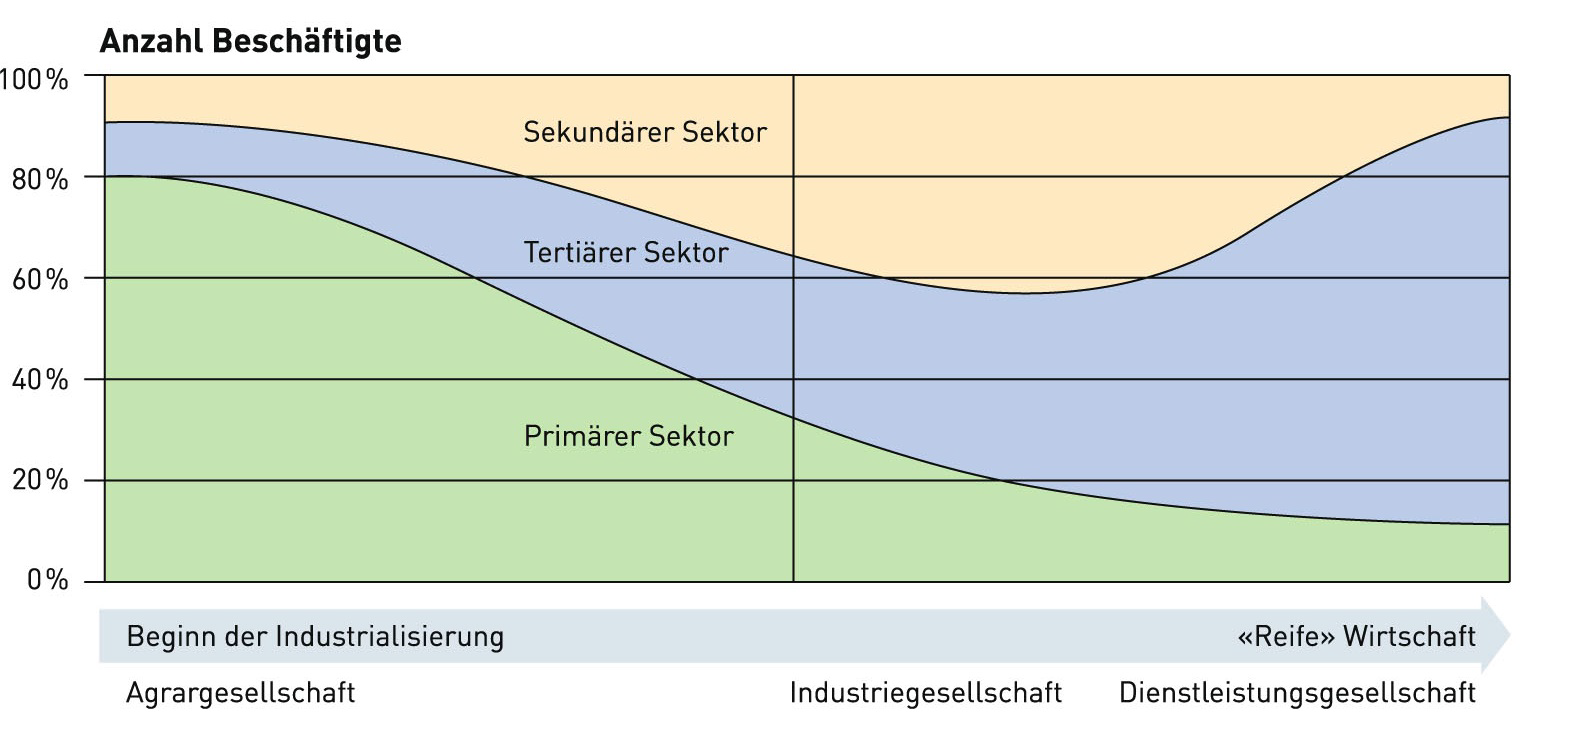
\includegraphics[width=\textwidth]{./resources/fourastie.png}
    \end{figure}
    \end{center}
\end{snippet}

\end{document}